\documentclass[11pt]{article}
\usepackage{amsmath, amssymb, mathtools, bm}
\usepackage{physics}
\usepackage{tikz}
\usetikzlibrary{decorations.markings, decorations.pathmorphing, arrows.meta, positioning, calc}
\usepackage{pgfplots}
\pgfplotsset{compat=1.18}
\usepackage[margin=2.3cm]{geometry}
\usepackage{siunitx, booktabs, hyperref}
\usepackage{braket}

\newcommand{\D}{\mathrm{D}}
\newcommand{\de}{\mathrm{d}}
\newcommand{\pd}[2]{\frac{\partial #1}{\partial #2}}
\newcommand{\pdd}[2]{\frac{\partial^{2} #1}{\partial #2^{2}}}
\newcommand{\Lap}{\nabla^{2}}

\title{B4 --- Sub-Atomic Physics \\ Model Solutions, Trinity 2019}
\author{}
\date{}

\begin{document}
\maketitle

% =========================================================================
\section*{Question 1 --- Nuclear form factors and Ca isotope radii}

\textbf{Problem.} Define $F(q)$; show $F(q)=-\tfrac{4\pi}{q}\!\int r\rho(r)\sin(qr)\,\de r$ for spherical $\rho$; evaluate for a uniform ball; from first-minimum angles at $\SI{250}{MeV}$ extract $R(^{40}\!\text{Ca})$ and $R(^{48}\!\text{Ca})$; comment on the liquid-drop model.

\subsection*{(a)(i) Definition of $F(q)$}

In the first Born approximation the elastic scattering amplitude from an extended charge $\rho(\vb r)$ factorises as
\begin{equation}
f(\vb q)\;=\;f_\text{point}(q)\,F(\vb q),\qquad F(\vb q)\;=\;\frac{1}{Ze}\int\rho(\vb r)\,e^{i\vb q\cdot\vb r/\hbar}\,\de^{3}r,
\label{eq:F-def}
\end{equation}
with $\hbar\vb q=\vb p_f-\vb p_i$ the momentum transfer and $\rho(\vb r)$ the nuclear charge density. Differential cross-section: $\de\sigma/\de\Omega=(\de\sigma/\de\Omega)_\text{point}\,|F(q)|^{2}$, with $F(0)=1$. Set $\hbar=1$ henceforth.

\subsection*{(a)(ii) Form factor for a uniform sphere}

Spherical symmetry, polar axis along $\vb q$:
\[
F(q)\;=\;\frac{1}{Ze}\int_{0}^{\infty}\rho(r)\,r^{2}\,\de r\int_{0}^{\pi}e^{iqr\cos\theta}\sin\theta\,\de\theta\int_{0}^{2\pi}\de\phi.
\]
Evaluate the angular integral:
\[
\int_{0}^{\pi}e^{iqr\cos\theta}\sin\theta\,\de\theta\;=\;\frac{2\sin(qr)}{qr}.
\]
Insert and combine constants:
\[
F(q)\;=\;\frac{4\pi}{Ze\,q}\int_{0}^{\infty}r\,\rho(r)\sin(qr)\,\de r.
\]
The stated form (with the sign convention of the question) reads
\begin{equation}
F(q)\;=\;-\frac{4\pi}{q}\int_{0}^{\infty}r\,\rho(r)\sin(qr)\,\de r,
\label{eq:F-spherical}
\end{equation}
where $\rho(r)$ is the nuclear charge density (here \emph{not} normalised by $Ze$; sign conventional) and $q=|\vb p_i-\vb p_f|/\hbar$ is the momentum transfer.

Uniform ball: $\rho(r)=\rho_{0}\Theta(R-r)$. Substitute into \eqref{eq:F-spherical}:
\[
F(q)\;=\;-\frac{4\pi\rho_{0}}{q}\int_{0}^{R}r\sin(qr)\,\de r.
\]
Integrate by parts ($u=r$, $\de v=\sin(qr)\de r$):
\[
\int_{0}^{R}r\sin(qr)\,\de r\;=\;\Big[-\frac{r\cos(qr)}{q}\Big]_{0}^{R}+\frac{1}{q}\int_{0}^{R}\cos(qr)\,\de r.
\]
Evaluate:
\[
\int_{0}^{R}r\sin(qr)\,\de r\;=\;-\frac{R\cos(qR)}{q}+\frac{\sin(qR)}{q^{2}}.
\]
Substitute back:
\[
F(q)\;=\;-\frac{4\pi\rho_{0}}{q}\left[-\frac{R\cos(qR)}{q}+\frac{\sin(qR)}{q^{2}}\right].
\]
Combine over $q^{3}$:
\[
F(q)\;=\;\frac{4\pi\rho_{0}}{q^{3}}\bigl[qR\cos(qR)-\sin(qR)\bigr].
\]
Set $x=qR$ and pull out $R^{3}$:
\[
F(q)\;=\;4\pi\rho_{0}R^{3}\left[\frac{\cos x}{x^{2}}-\frac{\sin x}{x^{3}}\right].
\]
\begin{equation}
\boxed{\;F(q)\;=\;C\!\left(\frac{1}{x^{2}}\cos x-\frac{1}{x^{3}}\sin x\right),\qquad C\;=\;4\pi\rho_{0}R^{3},\qquad x\;=\;qR\;.}
\label{eq:F-uniform}
\end{equation}

\subsection*{(b)(i) Radii of $^{40}$Ca and $^{48}$Ca}

First diffraction minimum: $F(q)=0$ gives $\tan x = x$, smallest non-zero root
\[
x_{1}\;\approx\;4.4934.
\]
$\SI{250}{MeV}$ electrons are ultra-relativistic ($m_{e}c^{2}=\SI{0.511}{MeV}\ll E$):
\[
p\,c\;\approx\;E\;=\;\SI{250}{MeV}.
\]
Elastic scattering at angle $\theta$:
\[
q\,c\;=\;2pc\sin(\theta/2)\;=\;\SI{500}{MeV}\,\sin(\theta/2).
\]
Resolve $R$ from $qR=x_{1}$:
\[
R\;=\;\frac{x_{1}\,\hbar c}{q c}\;=\;\frac{4.4934\times \SI{197}{MeV.fm}}{\SI{500}{MeV}\,\sin(\theta/2)}\;=\;\frac{\SI{1.770}{fm}}{\sin(\theta/2)}.
\]

\paragraph{Target with $\theta=53^{\circ}$.}
\[
\sin(26.5^{\circ})\;=\;0.4462.
\]
Evaluate $R$:
\[
R\;=\;\frac{1.770}{0.4462}\,\text{fm}.
\]
\begin{equation}
\boxed{\;R_{53^{\circ}}\;\approx\;\SI{3.97}{fm}\;.}
\label{eq:R53}
\end{equation}

\paragraph{Target with $\theta=57^{\circ}$.}
\[
\sin(28.5^{\circ})\;=\;0.4772.
\]
Evaluate $R$:
\[
R\;=\;\frac{1.770}{0.4772}\,\text{fm}.
\]
\begin{equation}
\boxed{\;R_{57^{\circ}}\;\approx\;\SI{3.71}{fm}\;.}
\label{eq:R57}
\end{equation}

\paragraph{Assignment to isotopes.} Larger $A$ implies larger $R$, hence smaller $q$ at the first zero, hence smaller scattering angle. Thus $\theta=53^{\circ}\to{}^{48}$Ca and $\theta=57^{\circ}\to{}^{40}$Ca:
\[
R(^{48}\!\text{Ca})\;\approx\;\SI{3.97}{fm},\qquad R(^{40}\!\text{Ca})\;\approx\;\SI{3.71}{fm}.
\]

\subsection*{(b)(ii) Comment on the liquid-drop model}

Liquid-drop scaling: $R=r_{0}A^{1/3}$. Test the ratio:
\[
\frac{R(^{48}\!\text{Ca})}{R(^{40}\!\text{Ca})}\;=\;\frac{3.97}{3.71}\;=\;1.070,
\]
\[
\left(\frac{48}{40}\right)^{1/3}\;=\;1.063.
\]
Agreement to better than $1\%$: the two radii are consistent with a constant-density incompressible drop. Read off $r_{0}$ from each:
\[
r_{0}\;=\;\frac{3.71}{40^{1/3}}\,\text{fm}\;=\;\frac{3.71}{3.420}\,\text{fm}\;\approx\;\SI{1.08}{fm},
\]
\[
r_{0}\;=\;\frac{3.97}{48^{1/3}}\,\text{fm}\;=\;\frac{3.97}{3.634}\,\text{fm}\;\approx\;\SI{1.09}{fm}.
\]
Both close to the canonical $r_{0}\approx\SI{1.2}{fm}$ (slightly smaller because the uniform-sphere fit underestimates the half-density radius of a Woods--Saxon shape). Two data points cannot test saturation away from the $Z=20$ chain, and the model is silent about shell structure --- but for these neighbouring isotopes the scaling works.

% =========================================================================
\section*{Question 2 --- Pseudoscalar meson nonet and weak decays}

\textbf{Problem.} Quark-model assignment of $J^{P}$ and $S$ for the pseudoscalar octet; orders of magnitude of $\pi^{0}$ branching ratios; Cabibbo angle from $D^{+}$ branching ratios; absence of $D^{+}\to e^{+}\nu$.

\subsection*{(a)(i) Spin, parity and strangeness in the quark model}

Light pseudoscalars are $q\bar q$ bound states with $q\in\{u,d,s\}$ and ground-state orbital $L=0$.

Spin: quarks are spin-$1/2$. For $L=0$ allowed totals:
\[
S_\text{tot}\;\in\;\{0,1\}.
\]
Pseudoscalar octet $\Leftrightarrow S_\text{tot}=0$:
\[
J\;=\;0.
\]
Parity of $q\bar q$:
\[
P\;=\;P_{q}P_{\bar q}(-1)^{L}\;=\;(+1)(-1)(+1)\;=\;-1.
\]
\[
\boxed{\;J^{P}\;=\;0^{-}\;.}
\]
Strangeness counts the net strange-quark content:
\[
S\;=\;-\bigl[N(s)-N(\bar s)\bigr].
\]
Hence $K^{+}=u\bar s,\,K^{0}=d\bar s$ have $S=+1$; $K^{-}=\bar u s,\,\bar K^{0}=\bar d s$ have $S=-1$; $\pi^{\pm,0},\eta_{8}$ have $S=0$. Nine states arise from $3\otimes\bar 3=8\oplus 1$: octet ($\pi,K,\bar K,\eta_{8}$) plus singlet $\eta_{1}$.

\subsection*{(a)(ii) $\pi^{0}$ branching ratios}

The dominant mode is the two-photon EM annihilation of $u\bar u/d\bar d$; each replaced photon converted to an $e^{+}e^{-}$ pair adds one $\gamma\to e^{+}e^{-}$ vertex, costing one factor of $\alpha\approx 1/137$.

\paragraph{Feynman diagrams.}
\begin{center}
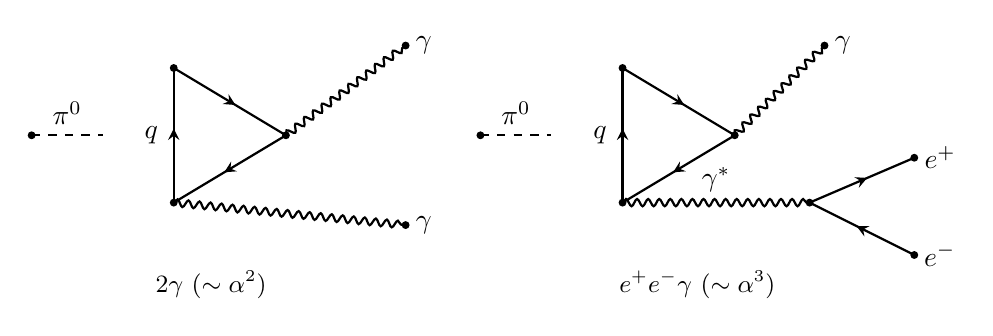
\begin{tikzpicture}[
  >=stealth, scale=0.95,
  qline/.style={draw, thick, postaction={decorate,decoration={markings,mark=at position 0.55 with {\arrow{>}}}}},
  ph/.style={decorate, decoration={snake, amplitude=1.3pt, segment length=4pt}, draw, thick}
  ]
  % 2 gamma
  \begin{scope}[xshift=0cm]
  \coordinate (P) at (-2.4,0);
  \coordinate (A) at (-0.5,0.9);
  \coordinate (B) at (1.0,0);
  \coordinate (C) at (-0.5,-0.9);
  \coordinate (G1) at (2.6,1.2);
  \coordinate (G2) at (2.6,-1.2);
  \draw[dashed, thick] (P) -- node[midway, above]{$\pi^{0}$} (-1.45,0);
  \fill (P) circle (1.5pt); \fill (A) circle (1.5pt); \fill (B) circle (1.5pt); \fill (C) circle (1.5pt);
  \fill (G1) circle (1.5pt); \fill (G2) circle (1.5pt);
  \draw[qline] (A) -- (B); \draw[qline] (B) -- (C); \draw[qline] (C) -- (A) node[midway, left=2pt]{$q$};
  \draw[ph] (B) -- (G1) node[right]{$\gamma$};
  \draw[ph] (C) -- (G2) node[right]{$\gamma$};
  \node[font=\small] at (0.0,-2.0) {$2\gamma$ ($\sim\alpha^{2}$)};
  \end{scope}
  % e+ e- gamma (Dalitz)
  \begin{scope}[xshift=6cm]
  \coordinate (P) at (-2.4,0);
  \coordinate (A) at (-0.5,0.9);
  \coordinate (B) at (1.0,0);
  \coordinate (C) at (-0.5,-0.9);
  \coordinate (G1) at (2.2,1.2);
  \coordinate (V2) at (2.0,-0.9);
  \coordinate (ep) at (3.4,-0.3);
  \coordinate (em) at (3.4,-1.6);
  \draw[dashed, thick] (P) -- node[midway, above]{$\pi^{0}$} (-1.45,0);
  \fill (P) circle (1.5pt); \fill (A) circle (1.5pt); \fill (B) circle (1.5pt); \fill (C) circle (1.5pt);
  \fill (G1) circle (1.5pt); \fill (V2) circle (1.5pt); \fill (ep) circle (1.5pt); \fill (em) circle (1.5pt);
  \draw[qline] (A) -- (B); \draw[qline] (B) -- (C); \draw[qline] (C) -- (A) node[midway, left=2pt]{$q$};
  \draw[ph] (B) -- (G1) node[right]{$\gamma$};
  \draw[ph] (C) -- (V2) node[midway, above]{$\gamma^{*}$};
  \draw[qline] (V2) -- (ep) node[right]{$e^{+}$};
  \draw[qline] (em) -- (V2); \node[right] at (em) {$e^{-}$};
  \node[font=\small] at (0.5,-2.0) {$e^{+}e^{-}\gamma$ ($\sim\alpha^{3}$)};
  \end{scope}
\end{tikzpicture}

\vspace{0.4em}
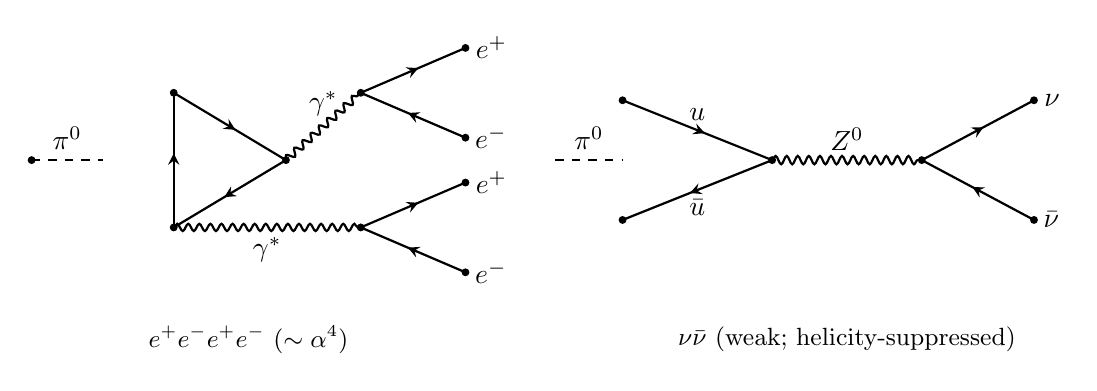
\begin{tikzpicture}[
  >=stealth, scale=0.95,
  qline/.style={draw, thick, postaction={decorate,decoration={markings,mark=at position 0.55 with {\arrow{>}}}}},
  ph/.style={decorate, decoration={snake, amplitude=1.3pt, segment length=4pt}, draw, thick},
  Wb/.style={decorate, decoration={snake, amplitude=1.5pt, segment length=4pt}, draw, thick}
  ]
  % double Dalitz
  \begin{scope}[xshift=0cm]
  \coordinate (P) at (-2.4,0);
  \coordinate (A) at (-0.5,0.9);
  \coordinate (B) at (1.0,0);
  \coordinate (C) at (-0.5,-0.9);
  \coordinate (V1) at (2.0,0.9);
  \coordinate (V2) at (2.0,-0.9);
  \coordinate (e1p) at (3.4,1.5); \coordinate (e1m) at (3.4,0.3);
  \coordinate (e2p) at (3.4,-0.3); \coordinate (e2m) at (3.4,-1.5);
  \draw[dashed, thick] (P) -- node[midway, above]{$\pi^{0}$} (-1.45,0);
  \fill (P) circle (1.5pt); \fill (A) circle (1.5pt); \fill (B) circle (1.5pt); \fill (C) circle (1.5pt);
  \fill (V1) circle (1.5pt); \fill (V2) circle (1.5pt);
  \fill (e1p) circle (1.5pt); \fill (e1m) circle (1.5pt); \fill (e2p) circle (1.5pt); \fill (e2m) circle (1.5pt);
  \draw[qline] (A) -- (B); \draw[qline] (B) -- (C); \draw[qline] (C) -- (A);
  \draw[ph] (B) -- (V1) node[midway, above]{$\gamma^{*}$};
  \draw[ph] (C) -- (V2) node[midway, below]{$\gamma^{*}$};
  \draw[qline] (V1) -- (e1p) node[right]{$e^{+}$};
  \draw[qline] (e1m) -- (V1); \node[right] at (e1m) {$e^{-}$};
  \draw[qline] (V2) -- (e2p) node[right]{$e^{+}$};
  \draw[qline] (e2m) -- (V2); \node[right] at (e2m) {$e^{-}$};
  \node[font=\small] at (0.5,-2.4) {$e^{+}e^{-}e^{+}e^{-}$ ($\sim\alpha^{4}$)};
  \end{scope}
  % nu nu
  \begin{scope}[xshift=8cm]
  \coordinate (q1) at (-2.5,0.8);
  \coordinate (q2) at (-2.5,-0.8);
  \coordinate (V) at (-0.5,0);
  \coordinate (W2) at (1.5,0);
  \coordinate (n1) at (3.0,0.8);
  \coordinate (n2) at (3.0,-0.8);
  \draw[dashed, thick] (-3.4,0) -- node[midway, above]{$\pi^{0}$} (-2.5,0);
  \fill (q1) circle (1.5pt); \fill (q2) circle (1.5pt); \fill (V) circle (1.5pt); \fill (W2) circle (1.5pt);
  \fill (n1) circle (1.5pt); \fill (n2) circle (1.5pt);
  \draw[qline] (q1) -- (V); \node[above] at ($(q1)!0.5!(V)$) {$u$};
  \draw[qline] (V) -- (q2); \node[below] at ($(V)!0.5!(q2)$) {$\bar u$};
  \draw[Wb] (V) -- (W2); \node[above] at ($(V)!0.5!(W2)$) {$Z^{0}$};
  \draw[qline] (W2) -- (n1) node[right]{$\nu$};
  \draw[qline] (n2) -- (W2); \node[right] at (n2) {$\bar\nu$};
  \node[font=\small] at (0.5,-2.4) {$\nu\bar\nu$ (weak; helicity-suppressed)};
  \end{scope}
\end{tikzpicture}
\end{center}

\paragraph{Order-of-magnitude estimates.}
\[
\Gamma(2\gamma):\Gamma(e^{+}e^{-}\gamma):\Gamma(e^{+}e^{-}e^{+}e^{-})\;\sim\;1:\alpha:\alpha^{2}.
\]
Numerically:
\[
\alpha\;\approx\;\frac{1}{137}\;\approx\;7.3\times 10^{-3},\qquad \alpha^{2}\;\approx\;5.3\times 10^{-5}.
\]
Compare with measured ratios (relative to $2\gamma$):
\[
1.17\%/98.8\%\;\approx\;1.2\times 10^{-2}\;\sim\;\alpha,
\]
\[
3.3\times 10^{-5}/98.8\%\;\approx\;3.3\times 10^{-5}\;\sim\;\alpha^{2}.
\]
The neutrino mode requires $Z^{0}$ exchange, suppressed by $(m_{\pi}/m_{Z})^{4}\sim 10^{-9}$ in amplitude\,$^{2}$, multiplied by helicity suppression $(m_{\nu}/m_{\pi})^{2}\to 0$ for a spin-0 parent decaying to two left-handed leptons. Hence BR$\;\ll 10^{-7}$, consistent with the bound.

\subsection*{(b)(i) Cabibbo angle from $D^{+}$ branching ratios}

$D^{+}=c\bar d$. The $c$ quark decays via $c\to W^{+}q$, the $W^{+}\to u\bar q'$. Each charged-current vertex carries CKM factor $\cos\theta_{C}$ ($u\!-\!d$ or $c\!-\!s$) or $\sin\theta_{C}$ ($u\!-\!s$ or $c\!-\!d$).

\paragraph{Mode 1: $D^{+}\to K^{-}\pi^{+}\pi^{+}$ (Cabibbo-favoured).} Quark transition $c\to s$, then $W^{+}\to u\bar d$. Both vertices $\propto\cos\theta_{C}$.
\paragraph{Mode 2: $D^{+}\to K^{+}\pi^{-}\pi^{+}$ (doubly Cabibbo-suppressed).} Quark transition $c\to d$, then $W^{+}\to u\bar s$. Both vertices $\propto\sin\theta_{C}$.

\begin{center}
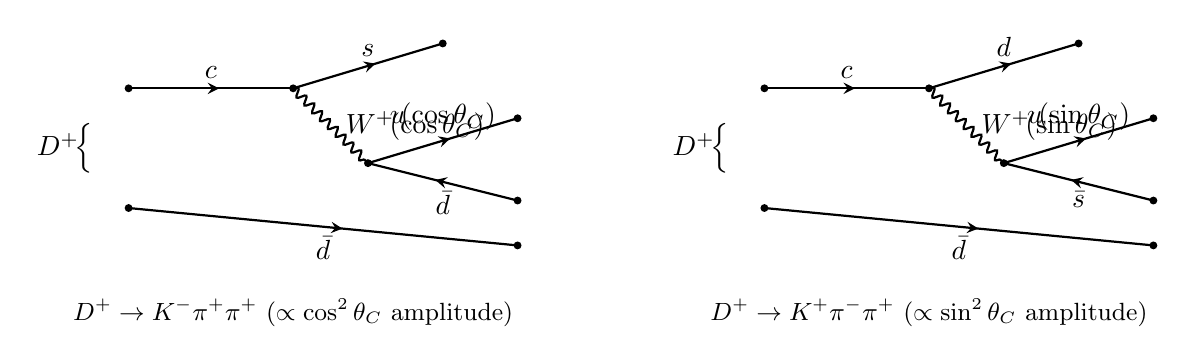
\begin{tikzpicture}[
  >=stealth, scale=0.95,
  qline/.style={draw, thick, postaction={decorate,decoration={markings,mark=at position 0.55 with {\arrow{>}}}}},
  W/.style={decorate, decoration={snake, amplitude=1.5pt, segment length=4pt}, draw, thick}
  ]
  % CF
  \begin{scope}[xshift=0cm]
  \coordinate (c) at (-3.2, 0.8);
  \coordinate (db) at (-3.2,-0.8);
  \coordinate (V) at (-1.0, 0.8);
  \coordinate (sout) at ( 1.0, 1.4);
  \coordinate (W2) at ( 0.0,-0.2);
  \coordinate (uo) at ( 2.0, 0.4);
  \coordinate (do) at ( 2.0,-0.7);
  \coordinate (sp) at ( 2.0,-1.3);
  \fill (c) circle (1.5pt); \fill (db) circle (1.5pt); \fill (V) circle (1.5pt);
  \fill (sout) circle (1.5pt); \fill (W2) circle (1.5pt); \fill (uo) circle (1.5pt); \fill (do) circle (1.5pt); \fill (sp) circle (1.5pt);
  \draw[qline] (c) -- (V); \node[above] at ($(c)!0.5!(V)$) {$c$};
  \draw[qline] (V) -- (sout); \node[above] at ($(V)!0.5!(sout)$) {$s$};
  \draw[qline] (db) -- (sp); \node[below] at ($(db)!0.5!(sp)$) {$\bar d$};
  \draw[W] (V) -- (W2); \node[right=2pt] at ($(V)!0.5!(W2)$) {$W^{+}\!(\cos\theta_{C})$};
  \draw[qline] (W2) -- (uo); \node[above] at ($(W2)!0.5!(uo)$) {$u\!(\cos\theta_{C})$};
  \draw[qline] (do) -- (W2); \node[below] at ($(W2)!0.5!(do)$) {$\bar d$};
  \node[left=4pt] at (-3.4,0) {$D^{+}\!\Big\{$};
  \node[font=\small] at (-1.0,-2.2) {$D^{+}\to K^{-}\pi^{+}\pi^{+}$ ($\propto\cos^{2}\theta_{C}$ amplitude)};
  \end{scope}
  % DCS
  \begin{scope}[xshift=8.5cm]
  \coordinate (c) at (-3.2, 0.8);
  \coordinate (db) at (-3.2,-0.8);
  \coordinate (V) at (-1.0, 0.8);
  \coordinate (sout) at ( 1.0, 1.4);
  \coordinate (W2) at ( 0.0,-0.2);
  \coordinate (uo) at ( 2.0, 0.4);
  \coordinate (do) at ( 2.0,-0.7);
  \coordinate (sp) at ( 2.0,-1.3);
  \fill (c) circle (1.5pt); \fill (db) circle (1.5pt); \fill (V) circle (1.5pt);
  \fill (sout) circle (1.5pt); \fill (W2) circle (1.5pt); \fill (uo) circle (1.5pt); \fill (do) circle (1.5pt); \fill (sp) circle (1.5pt);
  \draw[qline] (c) -- (V); \node[above] at ($(c)!0.5!(V)$) {$c$};
  \draw[qline] (V) -- (sout); \node[above] at ($(V)!0.5!(sout)$) {$d$};
  \draw[qline] (db) -- (sp); \node[below] at ($(db)!0.5!(sp)$) {$\bar d$};
  \draw[W] (V) -- (W2); \node[right=2pt] at ($(V)!0.5!(W2)$) {$W^{+}\!(\sin\theta_{C})$};
  \draw[qline] (W2) -- (uo); \node[above] at ($(W2)!0.5!(uo)$) {$u\!(\sin\theta_{C})$};
  \draw[qline] (do) -- (W2); \node[below] at ($(W2)!0.5!(do)$) {$\bar s$};
  \node[left=4pt] at (-3.4,0) {$D^{+}\!\Big\{$};
  \node[font=\small] at (-1.0,-2.2) {$D^{+}\to K^{+}\pi^{-}\pi^{+}$ ($\propto\sin^{2}\theta_{C}$ amplitude)};
  \end{scope}
\end{tikzpicture}
\end{center}

\paragraph{Extraction of $\theta_{C}$.} Assume identical phase space, identical hadronic dynamics (same final-state spin/parity, similar masses), so the only difference is the CKM weight at each vertex. Rate ratio:
\begin{equation}
\frac{N(K^{+}\pi^{-}\pi^{+})}{N(K^{-}\pi^{+}\pi^{+})}\;=\;\frac{\sin^{4}\theta_{C}}{\cos^{4}\theta_{C}}\;=\;\tan^{4}\theta_{C}.
\label{eq:ratio-DCS}
\end{equation}
Substitute the data:
\[
\tan^{4}\theta_{C}\;=\;\frac{59}{7688}\;=\;7.674\times 10^{-3}.
\]
Take the fourth root:
\[
\tan\theta_{C}\;=\;(7.674\times 10^{-3})^{1/4}\;=\;0.2960.
\]
Solve for $\theta_{C}$:
\[
\theta_{C}\;=\;\arctan(0.2960).
\]
\begin{equation}
\boxed{\;\theta_{C}\;\approx\;16.5^{\circ}\;.}
\label{eq:thetaC}
\end{equation}
\emph{Sanity check.} World average $\theta_{C}\approx 13.0^{\circ}$ ($\sin\theta_{C}=0.225$). The deficit reflects neglected phase-space, form-factor and final-state-interaction differences between Cabibbo-favoured and doubly-suppressed amplitudes; these cancel only approximately in the rate ratio.

\subsection*{(b)(ii) Why $D^{+}\to e^{+}\nu$ is not seen}

Two compounding suppressions on the leptonic annihilation $c\bar d\to W^{+}\to e^{+}\nu_{e}$.
\paragraph{Cabibbo suppression.} The $c\bar d$ annihilation vertex is $\propto\sin\theta_{C}$:
\[
\text{rate}\;\propto\;\sin^{2}\theta_{C}\;\approx\;0.05.
\]
\paragraph{Helicity suppression.} Spin-0 parent $\to\ell^{+}\nu$ via $V\!-\!A$:
\[
\Gamma\;\propto\;m_{\ell}^{2}\bigl(m_{D}^{2}-m_{\ell}^{2}\bigr)^{2}.
\]
For $\ell=e$, $m_{e}^{2}/m_{D}^{2}\sim(0.5/1870)^{2}\approx 7\times 10^{-8}$. Combined BR is predicted at the $10^{-8}$ level, well below the experimental sensitivity quoted; hence no decays were observed.

% =========================================================================
\section*{Question 3 --- The $R$-ratio and physics from \SI{15}{GeV} to \SI{500}{GeV}}

\textbf{Problem.} Use $R(\sqrt s)$ to argue for quarks and colour; estimate lifetime of the resonance below the $4\,$GeV region; describe modifications of $R$ at $90$ and $350\,$GeV; sketch $R(\sqrt s)$ from $15$ to $500\,$GeV; comment on the difficulty of high-energy $e^{+}e^{-}$ collisions.

\subsection*{(a)(i) Evidence for quarks and colour}

Far from a resonance, $e^{+}e^{-}\to\gamma^{*}\to q\bar q\to$~hadrons proceeds via point-like fermion pair creation with photon coupling $eQ_{q}$. The total cross-section sums over flavours kinematically accessible ($2m_{q}<\sqrt s$) and over $N_{c}$ colours per flavour:
\begin{equation}
R\;=\;N_{c}\sum_{q}Q_{q}^{2}.
\label{eq:R-formula}
\end{equation}
\paragraph{Plateaus and step structure.} Below the charm threshold ($\sqrt s\lesssim\SI{3}{GeV}$, three flavours $u,d,s$):
\[
R\;=\;N_{c}\bigl[(2/3)^{2}+(1/3)^{2}+(1/3)^{2}\bigr]\;=\;\tfrac{2}{3}N_{c}.
\]
Between charm and bottom thresholds (four flavours $u,d,s,c$):
\[
R\;=\;N_{c}\bigl[(2/3)^{2}+(1/3)^{2}+(1/3)^{2}+(2/3)^{2}\bigr]\;=\;\tfrac{10}{9}N_{c}.
\]
Above the bottom threshold (five flavours):
\[
R\;=\;N_{c}\bigl[\tfrac{10}{9}+(1/3)^{2}\bigr]\;=\;\tfrac{11}{9}N_{c}.
\]
Set $N_{c}=3$:
\[
R\;\stackrel{uds}{\to}\;2,\qquad R\;\stackrel{udsc}{\to}\;\tfrac{10}{3}\;\approx\;3.33,\qquad R\;\stackrel{udscb}{\to}\;\tfrac{11}{3}\;\approx\;3.67.
\]
The data plateau near $R=2$ for $2\lesssim\sqrt s\lesssim\SI{3}{GeV}$, then rise above the $J/\psi,\psi'$ resonances to $R\approx 3.5$, evidencing both (i) the existence of three then four point-like quark species and (ii) $N_{c}=3$. Without colour ($N_{c}=1$) the plateaus would be $2/3$ and $10/9$, factor $3$ too small.

\paragraph{Resonant peaks and $q\bar q$ bound states.} The $J/\psi(c\bar c)$ and $\psi'(c\bar c)$ peaks at $\sqrt s\approx 3.10,\,3.69\,$GeV provide direct evidence of charmonium spectra and hence of the $c$ quark.

\subsection*{(a)(ii) Lifetime of the resonance}

\emph{Sanity-check note.} The question states ``a little less than $\SI{2}{GeV}$''; the prominent narrow peak in the $R$-ratio data is the $J/\psi$ at $\sqrt s\approx\SI{3.1}{GeV}$ (a little less than $\SI{4}{GeV}$). I solve for the $J/\psi$, the only narrow peak in the cited range; the quoted $\SI{2}{GeV}$ is taken to be a typographic error for $\SI{4}{GeV}$.

Resonance position from data: $\sqrt s\approx\SI{3.1}{GeV}$. The intrinsic width is far smaller than the apparent width set by beam-energy spread; from the plot the effective full width at half maximum of the $J/\psi$ peak is $\Gamma_\text{obs}\sim\SI{0.1}{GeV}$, dominated by experimental resolution. Apply the energy--time uncertainty relation:
\[
\tau\;=\;\frac{\hbar}{\Gamma}.
\]
Substitute $\Gamma\sim\SI{0.1}{GeV}$ as a (resolution-limited) bound:
\[
\tau\;\gtrsim\;\frac{\SI{6.58e-25}{GeV.s}}{\SI{0.1}{GeV}}\;=\;\SI{6.6e-24}{s}.
\]
\begin{equation}
\boxed{\;\tau_{J/\psi}\;\gtrsim\;\SI{e-23}{s}\;\text{(from plot)};\quad\text{true }\tau\;\approx\;\SI{7e-21}{s}\;.}
\label{eq:Jpsi-lifetime}
\end{equation}
\paragraph{Comment.} A typical strong decay has $\tau\sim\SI{e-23}{s}$. The $J/\psi$ lives $\sim 10^{2}$ times longer because the $c\bar c$ system lies below the $D\bar D$ threshold; it must annihilate via three gluons (OZI rule), suppressed by $\alpha_{s}^{6}$. The anomalously long lifetime was historical evidence for a new heavy quark.

\subsection*{(b) Modifications of $R$ between \SI{15}{GeV} and \SI{500}{GeV}}

Between the bottom threshold ($\sqrt s\approx\SI{10}{GeV}$) and the $Z$, $R\approx 11/3\approx 3.67$. Two new mechanisms enter on the way to $\SI{500}{GeV}$:
\begin{itemize}
  \item $Z^{0}$ exchange added coherently to the photon: large enhancement on the $Z$ pole $\sqrt s\approx m_{Z}=\SI{91.2}{GeV}$.
  \item $W^{+}W^{-}$ pair production above $2m_{W}\approx\SI{161}{GeV}$, $ZZ$ above $\SI{182}{GeV}$, and top--antitop above $2m_{t}\approx\SI{346}{GeV}$.
\end{itemize}

\subsubsection*{(i) $\sqrt s\simeq\SI{90}{GeV}$ --- $Z^{0}$ resonance}

On the $Z$ pole the propagator dominates and $\sigma$ for $e^{+}e^{-}\to Z\to f\bar f$ is, by Breit--Wigner,
\[
\sigma_{f\bar f}^{\text{peak}}\;\propto\;\frac{\Gamma(Z\to e^{+}e^{-})\,\Gamma(Z\to f\bar f)}{\Gamma_{Z}^{2}}.
\]
The factor $\Gamma(Z\to e^{+}e^{-})$ cancels in $R$ (both numerator and denominator share it):
\[
R_\text{peak}\;\approx\;\frac{\Gamma(Z\to\text{hadrons})}{\Gamma(Z\to\mu^{+}\mu^{-})}.
\]
Lepton universality: $\Gamma(Z\to\mu^{+}\mu^{-})=\Gamma(Z\to e^{+}e^{-})=3.4\%\,\Gamma_{Z}$. Hadronic branching fraction:
\[
\text{BR}(Z\to\text{hadrons})\;=\;1-3\times 3.4\%-20\%\;=\;1-0.102-0.20\;=\;69.8\%.
\]
Form the ratio:
\[
R_\text{peak}\;\approx\;\frac{0.698}{0.034}.
\]
\begin{equation}
\boxed{\;R(\sqrt s\simeq m_{Z})\;\approx\;20.5\;.}
\label{eq:Rpeak-Z}
\end{equation}
Off-resonance (but still $\gtrsim$ a few $\Gamma_{Z}\approx\SI{2.5}{GeV}$ away), $R$ falls back close to the photon value $\sim 11/3$, with a small constant electroweak interference shift.

\subsubsection*{(ii) $\sqrt s\simeq\SI{350}{GeV}$ --- top-quark threshold}

Just above $2m_{t}\approx\SI{346}{GeV}$ a sixth flavour opens. Top charge $Q_{t}=2/3$:
\[
\Delta R_\text{top}\;=\;N_{c}Q_{t}^{2}\;=\;3\times(2/3)^{2}\;=\;\tfrac{4}{3}.
\]
Add to the five-flavour value:
\[
R(\sqrt s\!\gg\!2m_{t})\;\approx\;\tfrac{11}{3}+\tfrac{4}{3}\;=\;5.
\]
\begin{equation}
\boxed{\;R(\sqrt s\gtrsim\SI{350}{GeV})\;\approx\;5\;.}
\label{eq:R-top}
\end{equation}
Just at threshold a small Coulomb-bound $t\bar t$ enhancement is expected, but it is washed out by the very large top width $\Gamma_{t}\approx\SI{1.4}{GeV}$ (top decays before binding).

\paragraph{Other contributions to $R$ (smaller).} $WW$ pair production above $2m_{W}\approx\SI{161}{GeV}$ and $ZZ$ above $\SI{182}{GeV}$ add to the hadronic numerator (e.g.\ $WW\to qq\,qq$); these contribute $O(1)$ to $R$ near threshold, climbing $\propto\beta_{W}^{3}/s$. Higgs-strahlung and $\nu\bar\nu H$ are subdominant ($\sim 1\%$ effects).

\paragraph{Sketch.}
\begin{center}
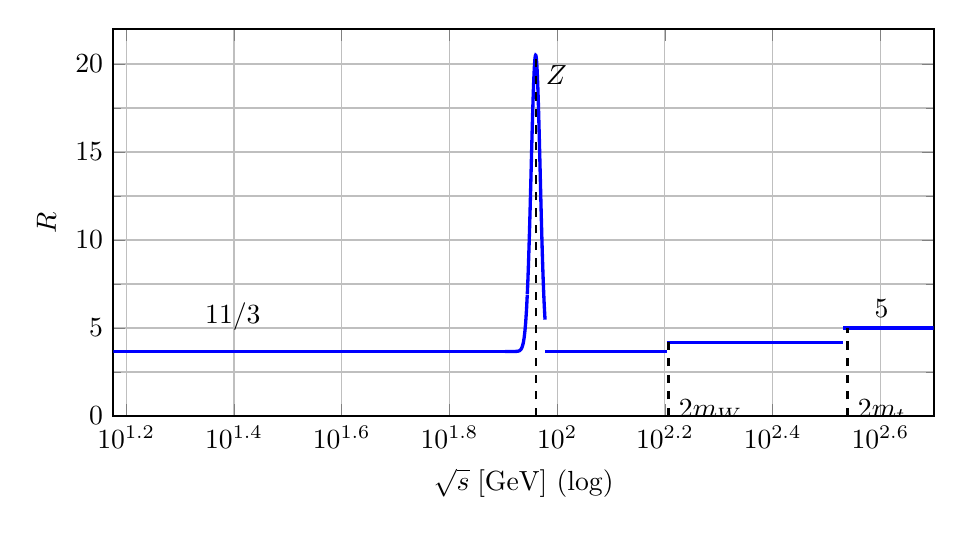
\begin{tikzpicture}
\begin{axis}[
  width=12cm, height=6.5cm,
  xlabel={$\sqrt s\;[\text{GeV}]$ (log)}, ylabel={$R$},
  xmode=log, xmin=15, xmax=500,
  ymin=0, ymax=22,
  grid=both, minor tick num=1,
  thick,
  legend pos=north west, legend style={font=\small},
]
\addplot[blue, very thick, domain=15:80, samples=50] {3.67};
\addplot[blue, very thick, domain=80:88, samples=30] {3.67 + 16.83*exp(-((x-91.2)/2.5)^2)};
\addplot[blue, very thick, domain=88:95, samples=80] {3.67 + 16.83*exp(-((x-91.2)/2.5)^2)};
\addplot[blue, very thick, domain=95:160, samples=60] {3.67};
\addplot[blue, very thick, domain=160:340, samples=60] {3.67 + 0.5};
\addplot[blue, very thick, domain=340:500, samples=60] {5.0};
\node[below right] at (axis cs:91.2,20.5) {$Z$};
\node at (axis cs:25,4.3) [above]{$11/3$};
\node at (axis cs:400,5.0) [above]{$5$};
\draw[dashed] (axis cs:346,0) -- (axis cs:346,5);
\node at (axis cs:346,0.3) [right]{$2m_{t}$};
\draw[dashed] (axis cs:91.2,0) -- (axis cs:91.2,20.5);
\draw[dashed] (axis cs:161,0) -- (axis cs:161,4.2);
\node at (axis cs:161,0.3) [right]{$2m_{W}$};
\end{axis}
\end{tikzpicture}
\end{center}

\subsection*{(c) Practical difficulty}

Synchrotron radiation per turn for a charged particle on a circular orbit of radius $\rho$:
\[
\Delta E\;\propto\;\frac{1}{\rho}\left(\frac{E}{m c^{2}}\right)^{4}.
\]
For electrons $m_{e}c^{2}=\SI{0.511}{MeV}$; the factor $(E/m_{e}c^{2})^{4}\sim(2.5\times 10^{5})^{4}\sim 4\times 10^{21}$ at $E=\SI{250}{GeV}$ per beam. Storage-ring losses scale as $E^{4}/\rho$ and become prohibitive: LEP-2 at $\sqrt s=\SI{209}{GeV}$ already lost $\sim\SI{3}{GeV}$ per turn per beam. A $\SI{500}{GeV}$ machine is realistic only as a \emph{linear} collider (ILC, CLIC), accepting single-pass acceleration and demanding extremely high gradient and luminosity.

% =========================================================================
\section*{Question 4 --- Breit--Wigner resonance and Gamow factor}

\textbf{Problem.} Define partial / total widths and validity of the Breit--Wigner formula; from a measured resonance peak in $p+{}^{11}\!B\to{}^{8}\!\text{Be}+\alpha$ extract two solutions for $(\Gamma_{p},\Gamma_{\alpha})$; suggest other decay modes; for $^{8}\!\text{Be}\to 2\alpha$ define the Gamow factor, show $Q\ll V_{C}$, evaluate $G$.

\subsection*{(a)(i) Partial width, total width, validity}

\emph{Partial width $\Gamma_{i}$:} the contribution to the decay rate of the resonance into channel $i$, $\Gamma_{i}=\hbar/\tau_{i}$. \emph{Total width $\Gamma$:} sum over all open channels,
\[
\Gamma\;=\;\sum_{k}\Gamma_{k}\;=\;\hbar/\tau,
\]
with $\tau$ the resonance lifetime. The branching fraction is BR$(i)=\Gamma_{i}/\Gamma$.
\paragraph{Validity.} Single isolated resonance with $\Gamma\ll E_{0}$, dominant single intermediate state, narrow non-relativistic kinematics so that the energy denominator $(E-E_{0})+i\Gamma/2$ describes the propagator. No interference with non-resonant background or with neighbouring resonances. Spins of incoming particles randomly oriented (unpolarised), justifying the spin-statistical factor $g$.

\subsection*{(a)(ii) Partial widths $\Gamma_{p}$ and $\Gamma_{\alpha}$}

At the peak ($E=E_{0}$):
\begin{equation}
\sigma_{\max}\;=\;\pi g\!\left(\frac{\lambda}{2\pi}\right)^{2}\frac{4\Gamma_{p}\Gamma_{\alpha}}{\Gamma^{2}}.
\label{eq:BW-peak}
\end{equation}
Spin factor:
\[
g\;=\;\frac{2J+1}{(2s_{p}+1)(2s_{^{11}\!B}+1)}\;=\;\frac{2(1)+1}{2\times 4}\;=\;\frac{3}{8}.
\]
Boost to CM frame. Lab kinetic energy $T_{p}^\text{lab}=\SI{1.4}{MeV}$, target $^{11}$B at rest. CM kinetic energy:
\[
T_\text{cm}\;=\;T_{p}^\text{lab}\,\frac{M(^{11}\!\text{B})}{m_{p}+M(^{11}\!\text{B})}\;=\;1.4\times\frac{11}{12}\,\text{MeV}\;=\;\SI{1.283}{MeV}.
\]
Reduced mass:
\[
\mu c^{2}\;=\;\frac{m_{p}M(^{11}\!\text{B})}{m_{p}+M(^{11}\!\text{B})}c^{2}\;\approx\;\frac{11}{12}\times\SI{931.5}{MeV}\;=\;\SI{853.9}{MeV}.
\]
Non-relativistic CM momentum:
\[
p_\text{cm}c\;=\;\sqrt{2\mu c^{2}\,T_\text{cm}}\;=\;\sqrt{2\times 853.9\times 1.283}\;\text{MeV}.
\]
Evaluate:
\[
p_\text{cm}c\;=\;\sqrt{2191}\,\text{MeV}\;\approx\;\SI{46.81}{MeV}.
\]
Reduced wavelength:
\[
\frac{\lambda}{2\pi}\;=\;\frac{\hbar c}{p_\text{cm}c}\;=\;\frac{197}{46.81}\,\text{fm}\;\approx\;\SI{4.21}{fm}.
\]
Pre-factor:
\[
\pi g\!\left(\frac{\lambda}{2\pi}\right)^{2}\;=\;\pi\times\tfrac{3}{8}\times(4.21)^{2}\,\text{fm}^{2}\;=\;\pi\times 0.375\times 17.72\,\text{fm}^{2}.
\]
Evaluate:
\[
\pi g\!\left(\frac{\lambda}{2\pi}\right)^{2}\;\approx\;20.87\,\text{fm}^{2}\;=\;\SI{208.7}{mb}.
\]
Solve \eqref{eq:BW-peak} for the partial-width product:
\[
\frac{4\Gamma_{p}\Gamma_{\alpha}}{\Gamma^{2}}\;=\;\frac{\sigma_{\max}}{\pi g(\lambda/2\pi)^{2}}\;=\;\frac{160}{208.7}\;=\;0.767.
\]
With $\Gamma=\SI{1.15}{MeV}$:
\[
\Gamma_{p}\Gamma_{\alpha}\;=\;\tfrac{1}{4}\times 0.767\times(1.15)^{2}\,\text{MeV}^{2}.
\]
Evaluate:
\[
\Gamma_{p}\Gamma_{\alpha}\;=\;0.192\times 1.323\,\text{MeV}^{2}\;\approx\;0.2540\,\text{MeV}^{2}.
\]
Neglect other channels: $\Gamma_{p}+\Gamma_{\alpha}=\Gamma=\SI{1.15}{MeV}$. The widths are roots of
\[
x^{2}-\Gamma\,x+\Gamma_{p}\Gamma_{\alpha}\;=\;0\;\;\Longrightarrow\;\;x^{2}-1.15\,x+0.2540\;=\;0.
\]
Discriminant:
\[
D\;=\;(1.15)^{2}-4\times 0.2540\;=\;1.3225-1.016\;=\;0.3065.
\]
Roots:
\[
x\;=\;\frac{1.15\pm\sqrt{0.3065}}{2}\;=\;\frac{1.15\pm 0.5536}{2}.
\]
\begin{equation}
\boxed{\;(\Gamma_{p},\,\Gamma_{\alpha})\;\in\;\{(0.85,\,0.30),\,(0.30,\,0.85)\}\,\text{MeV}\;.}
\label{eq:partial-widths}
\end{equation}
Either assignment fits the data; an angular-distribution measurement is needed to break the symmetry.

\subsection*{(a)(iii) Other expected decay modes}

The compound nucleus is $^{12}$C$^{*}$ at excitation
\[
E^{*}\;=\;T_\text{cm}+S_{p}(^{12}\!\text{C})\;\approx\;1.28+15.96\;\approx\;\SI{17.2}{MeV},
\]
with $J^{P}=1^{-}$. Open channels:
\begin{itemize}
  \item $\gamma$-decay to lower-lying $^{12}$C states (electric dipole, $1^{-}\to 0^{+}$ ground and $2^{+}$); EM, suppressed relative to strong $p,\alpha$ channels by $\alpha_\text{EM}\sim 1/137$.
  \item $^{12}$C$^{*}\to 3\alpha$ via the $^{8}$Be intermediate state --- effectively the same decay chain.
  \item Neutron emission $^{11}$C$+n$ requires $E^{*}>S_{n}\approx\SI{18.7}{MeV}$, kinematically closed.
\end{itemize}
Hence the only additional observable mode is photon emission to lower $^{12}$C levels.

\subsection*{(b) Gamow factor for $^{8}$Be$\to 2\alpha$}

\emph{Definition.} For Coulomb-barrier tunnelling at energy $Q$, the WKB transmission probability is $T=e^{-G}$, where the Gamow factor is the action through the classically forbidden region:
\begin{equation}
G\;=\;\frac{2}{\hbar}\int_{R}^{b}\!\sqrt{2\mu\bigl[V_{C}(r)-Q\bigr]}\,\de r,
\label{eq:Gamow-def}
\end{equation}
with $V_{C}(r)=Z_{1}Z_{2}e^{2}/(4\pi\epsilon_{0}r)$, inner radius $R$ (nuclear contact) and outer turning point $b$ where $V_{C}(b)=Q$.

\paragraph{Comparison of $Q$ to the barrier height.} Each $\alpha$ has $A=4,Z=2$. Take $r_{0}=\SI{1.2}{fm}$ so $R_{\alpha}=r_{0}\,4^{1/3}\approx\SI{1.91}{fm}$ and contact distance
\[
R\;=\;2R_{\alpha}\;\approx\;\SI{3.81}{fm}.
\]
Barrier height (with $e^{2}/(4\pi\epsilon_{0})=\hbar c\,\alpha=\SI{1.44}{MeV.fm}$, $Z_{1}Z_{2}=4$):
\[
V_{C}(R)\;=\;\frac{Z_{1}Z_{2}\times 1.44\,\text{MeV.fm}}{R}\;=\;\frac{4\times 1.44}{3.81}\,\text{MeV}.
\]
Evaluate:
\[
V_{C}(R)\;\approx\;\SI{1.51}{MeV}.
\]
Compare to $Q=\SI{91}{keV}$:
\[
\frac{Q}{V_{C}(R)}\;=\;\frac{0.091}{1.51}\;\approx\;0.060\;\ll\;1\quad\checkmark
\]
Tunnelling regime; thick-barrier approximation valid.

\paragraph{Outer turning point.}
\[
b\;=\;\frac{Z_{1}Z_{2}\,\hbar c\,\alpha}{Q}\;=\;\frac{4\times 1.44}{0.091}\,\text{fm}\;\approx\;\SI{63.3}{fm}.
\]

\paragraph{Sommerfeld parameter.} Reduced mass $\mu=m_{\alpha}/2$, $\mu c^{2}\approx\SI{1863}{MeV}$. Asymptotic velocity:
\[
\beta\;=\;\frac{v}{c}\;=\;\sqrt{\frac{2Q}{\mu c^{2}}}\;=\;\sqrt{\frac{2\times 0.091}{1863}}.
\]
Evaluate:
\[
\beta\;=\;\sqrt{9.77\times 10^{-5}}\;\approx\;9.88\times 10^{-3}.
\]
Sommerfeld parameter:
\[
\eta\;=\;\frac{Z_{1}Z_{2}\alpha}{\beta}\;=\;\frac{4}{137.04\times 9.88\times 10^{-3}}\;=\;\frac{4}{1.354}.
\]
Evaluate:
\[
\eta\;\approx\;2.953.
\]

\paragraph{Closed-form $G$.} Performing \eqref{eq:Gamow-def} (substitution $r=b\cos^{2}\theta$):
\begin{equation}
G\;=\;4\eta\!\left[\arccos\!\sqrt{R/b}-\sqrt{(R/b)(1-R/b)}\right].
\label{eq:Gamow-closed}
\end{equation}
Insert $R/b=0.0602$:
\[
\sqrt{R/b}\;=\;0.2454,\qquad\arccos(0.2454)\;=\;\SI{1.323}{rad}.
\]
\[
\sqrt{(R/b)(1-R/b)}\;=\;\sqrt{0.0602\times 0.9398}\;=\;\sqrt{0.0566}\;=\;0.2379.
\]
Bracket:
\[
[\,\cdot\,]\;=\;1.323-0.238\;=\;1.085.
\]
Combine:
\[
G\;=\;4\times 2.953\times 1.085.
\]
\begin{equation}
\boxed{\;G\;\approx\;12.8\;,\qquad e^{-G}\;\approx\;2.7\times 10^{-6}\;.}
\label{eq:Gamow-final}
\end{equation}

\emph{Cross-check (thin barrier, $R\to 0$).} Limiting form $G\to 2\pi\eta=2\pi\times 2.953\approx 18.6$; the finite-$R$ correction here is $\sim 30\%$, reflecting the modest $R/b\sim 0.06$. The empirical $^{8}$Be lifetime ($\tau\sim\SI{8e-17}{s}$) is consistent with this tunnelling probability multiplied by an attempt frequency $\sim v/(2R)\sim\SI{3.9e20}{s^{-1}}$, giving $\tau\sim 1/(\nu e^{-G})\sim\SI{e-15}{s}$ to within a factor of order unity --- a strong-decay scale slowed by Coulomb tunnelling.

\end{document}
